\documentclass[handout]{beamer}

\usepackage{color}
\usepackage{graphicx}
\usepackage{tikz}
\usepackage{multicol}
\usepackage{bm}

\title{Learning R}
\author{Patrick Lam}
\date{}

\newcommand{\red}{\color{red}}
\newcommand{\black}{\color{black}}

\usepackage{Sweave}
\begin{document}
\maketitle


\begin{frame}
\frametitle{setting up}
\pause
\begin{itemize}
\item download R from CRAN
\item work in the console (code not saved)
\item open a script, type code in script, and save as a .R file
\end{itemize}
\end{frame}

\begin{frame}
\begin{center}
Example code is in \red{red}
\end{center}
\end{frame}

\begin{frame}[fragile]
\frametitle{R as calculator}
\pause
\red
\begin{Schunk}
\begin{Sinput}
> 5 + 4
\end{Sinput}
\begin{Soutput}
[1] 9
\end{Soutput}
\end{Schunk}
\pause
\bigskip 
\begin{Schunk}
\begin{Sinput}
> 8 * 2 - sqrt(9)
\end{Sinput}
\begin{Soutput}
[1] 13
\end{Soutput}
\end{Schunk}
\pause
\bigskip
\begin{Schunk}
\begin{Sinput}
> log(4)/9^2
\end{Sinput}
\begin{Soutput}
[1] 0.01711475
\end{Soutput}
\end{Schunk}
\end{frame}

\begin{frame}[fragile]
\frametitle{objects}
R is an object-oriented programming language.  \pause Use \red\verb <- \black\hspace{1pt} as assignment operator for objects.
\pause
\bigskip
\red
\begin{Schunk}
\begin{Sinput}
> 5 + 4
\end{Sinput}
\begin{Soutput}
[1] 9
\end{Soutput}
\end{Schunk}
\pause
\begin{Schunk}
\begin{Sinput}
> my.sum <- 5 + 4
> my.sum
\end{Sinput}
\begin{Soutput}
[1] 9
\end{Soutput}
\end{Schunk}
\pause
\bigskip
\begin{Schunk}
\begin{Sinput}
> my.name <- "Patrick"
> my.name
\end{Sinput}
\begin{Soutput}
[1] "Patrick"
\end{Soutput}
\end{Schunk}
\black
\end{frame}

\begin{frame}[fragile]
\frametitle{vectors}
All objects consist of one or more \textbf{vectors}. \\
\pause
\bigskip
vector: a combination of elements (i.e. numbers, words), usually created using \red{\tt c()}\black, \red{\tt seq()}\black, or \red{\tt rep()}\black
\end{frame}

\begin{frame}[fragile]
\red
\begin{Schunk}
\begin{Sinput}
> empty.vector <- c()
> empty.vector
\end{Sinput}
\begin{Soutput}
NULL
\end{Soutput}
\end{Schunk}
\pause
\bigskip
\begin{Schunk}
\begin{Sinput}
> one.to.five <- c(1, 2, 3, 4, 5)
> one.to.five
\end{Sinput}
\begin{Soutput}
[1] 1 2 3 4 5
\end{Soutput}
\end{Schunk}
\pause
\bigskip
\begin{Schunk}
\begin{Sinput}
> poli.sci <- c("theory", "amer.", "comp.", "ir")
> poli.sci
\end{Sinput}
\begin{Soutput}
[1] "theory" "amer."  "comp."  "ir"    
\end{Soutput}
\end{Schunk}
\end{frame}

\begin{frame}[fragile]
\red
\begin{Schunk}
\begin{Sinput}
> one.to.ten <- 1:10
> one.to.ten
\end{Sinput}
\begin{Soutput}
 [1]  1  2  3  4  5  6  7  8  9 10
\end{Soutput}
\end{Schunk}
\pause
\bigskip
\begin{Schunk}
\begin{Sinput}
> two.to.five <- seq(from = 2, to = 5, by = 1)
> two.to.five
\end{Sinput}
\begin{Soutput}
[1] 2 3 4 5
\end{Soutput}
\end{Schunk}
\pause
\bigskip
\begin{Schunk}
\begin{Sinput}
> all.fours <- rep(4, times = 5)
> all.fours
\end{Sinput}
\begin{Soutput}
[1] 4 4 4 4 4
\end{Soutput}
\end{Schunk}
\end{frame}

\begin{frame}
\begin{center}
All elements in a vector must be of the same data type!
\end{center}
\end{frame}

\section{Data Types}
\begin{frame}
\frametitle{data types}
\begin{itemize}
\item numeric
\item character
\item logical
\end{itemize}
\end{frame}

\begin{frame}[fragile]
numeric: numbers
\pause
\bigskip
\red
\begin{Schunk}
\begin{Sinput}
> three <- 3
> three
\end{Sinput}
\begin{Soutput}
[1] 3
\end{Soutput}
\end{Schunk}
\pause
\bigskip
\begin{Schunk}
\begin{Sinput}
> is.numeric(three)
\end{Sinput}
\begin{Soutput}
[1] TRUE
\end{Soutput}
\end{Schunk}
\pause
\bigskip
\begin{Schunk}
\begin{Sinput}
> as.numeric("3")
\end{Sinput}
\begin{Soutput}
[1] 3
\end{Soutput}
\end{Schunk}
\black
\end{frame}

\begin{frame}[fragile]
character: for example, words or phrases (must be in "")
\pause
\bigskip
\red
\begin{Schunk}
\begin{Sinput}
> president <- "Barack Obama"
> president
\end{Sinput}
\begin{Soutput}
[1] "Barack Obama"
\end{Soutput}
\end{Schunk}
\pause
\bigskip
\begin{Schunk}
\begin{Sinput}
> is.character(president)
\end{Sinput}
\begin{Soutput}
[1] TRUE
\end{Soutput}
\end{Schunk}
\pause
\bigskip
\begin{Schunk}
\begin{Sinput}
> as.character(3)
\end{Sinput}
\begin{Soutput}
[1] "3"
\end{Soutput}
\end{Schunk}
\black
\end{frame}

\begin{frame}[fragile]
logical: {\tt TRUE (T)} or {\tt FALSE (F)}
\pause
\bigskip
\red
\begin{Schunk}
\begin{Sinput}
> num.vec <- c(5, 6, 4)
> logical.vec <- num.vec == 6
> logical.vec
\end{Sinput}
\begin{Soutput}
[1] FALSE  TRUE FALSE
\end{Soutput}
\end{Schunk}
\pause
\begin{Schunk}
\begin{Sinput}
> is.logical(logical.vec)
\end{Sinput}
\begin{Soutput}
[1] TRUE
\end{Soutput}
\end{Schunk}
\pause
\black
\bigskip
can also be represented as numeric 1 or 0:
\pause
\red
\bigskip
\begin{Schunk}
\begin{Sinput}
> as.numeric(logical.vec)
\end{Sinput}
\begin{Soutput}
[1] 0 1 0
\end{Soutput}
\end{Schunk}
\black
\end{frame}

\begin{frame}[fragile]
\begin{center}
All elements in a vector must be of the same data type!
\end{center}
\pause
\begin{itemize}
\item if a vector has a character element, all elements become character
\pause
\red
\begin{Schunk}
\begin{Sinput}
> mixed.vec <- c(5, "Patrick", TRUE)
> mixed.vec
\end{Sinput}
\begin{Soutput}
[1] "5"       "Patrick" "TRUE"   
\end{Soutput}
\end{Schunk}
\black
\pause
\bigskip
\item if a vector has both numeric and logical elements, all elements become numeric
\pause
\red
\begin{Schunk}
\begin{Sinput}
> mixed.vec2 <- c(10, FALSE)
> mixed.vec2
\end{Sinput}
\begin{Soutput}
[1] 10  0
\end{Soutput}
\end{Schunk}
\black
\pause
\bigskip
\end{itemize}
\begin{center}
character $>$ numeric $>$ logical
\end{center}

\end{frame}

\section{Object Classes}
\begin{frame}
\frametitle{object classes}
All objects consist of one or more vectors. \\
\pause
\bigskip
In addition to vector, objects can be of one of the following classes:
\pause
\begin{itemize}
\item matrix
\item array
\item dataframe
\item list
\end{itemize}
\end{frame}

\begin{frame}[fragile]
\frametitle{matrix}
A matrix is a two-dimensional ($r \times c$) object (think a bunch of stacked or side-by-side vectors).
\pause
\bigskip
\red
\begin{Schunk}
\begin{Sinput}
> a.matrix <- matrix(c(1, 2, 3, 4), nrow = 2, ncol = 2)
> a.matrix
\end{Sinput}
\begin{Soutput}
     [,1] [,2]
[1,]    1    3
[2,]    2    4
\end{Soutput}
\end{Schunk}
\pause
\begin{Schunk}
\begin{Sinput}
> class(a.matrix)
\end{Sinput}
\begin{Soutput}
[1] "matrix"
\end{Soutput}
\end{Schunk}
\black
\pause
\bigskip
\begin{center}
 All elements in a matrix must be of the same data type. \\
 \pause
 character $>$ numeric $>$ logical
 \end{center}
\end{frame}

\begin{frame}[fragile]
\frametitle{array}
An array is a three-dimensional ($r \times c \times h$) object (think a bunch of stacked $r \times c$ matrices). \\
\pause
\bigskip
All elements in an array must be of the same data type (character $>$ numeric $>$ logical).
\end{frame}

\begin{frame}[fragile]
\footnotesize
\red
\begin{Schunk}
\begin{Sinput}
> an.array <- array(0, dim = c(2, 2, 3))
> an.array
\end{Sinput}
\begin{Soutput}
, , 1

     [,1] [,2]
[1,]    0    0
[2,]    0    0

, , 2

     [,1] [,2]
[1,]    0    0
[2,]    0    0

, , 3

     [,1] [,2]
[1,]    0    0
[2,]    0    0
\end{Soutput}
\end{Schunk}
\normalsize
\end{frame}

\begin{frame}
\frametitle{dataframe}
A dataframe is a two-dimensional ($r \times c$) object (like a matrix).
\pause
\begin{itemize}
\item each column must be of the same data type, but data type may vary by column
\pause
\item regression and other statistical functions usually use dataframes
\pause
\item use \red{\tt as.data.frame()} \black to convert matrices to dataframes 
\end{itemize}
\end{frame}

\begin{frame}
\frametitle{list}
A list is a set of objects.\\
\pause
\bigskip
Each element in a list can be a(n):
\begin{itemize}
\item vector
\item matrix
\item array
\item dataframe
\item list
\end{itemize}
\end{frame}

\begin{frame}[fragile]
\red
\footnotesize
\begin{Schunk}
\begin{Sinput}
> a.vec <- 6:10
> a.matrix <- matrix(3, nrow = 2, ncol = 2)
> a.dataframe <- as.data.frame(a.matrix)
> a.list <- list(a.vec, a.matrix, a.dataframe)
> a.list
\end{Sinput}
\begin{Soutput}
[[1]]
[1]  6  7  8  9 10

[[2]]
     [,1] [,2]
[1,]    3    3
[2,]    3    3

[[3]]
  V1 V2
1  3  3
2  3  3
\end{Soutput}
\end{Schunk}
\black
\normalsize
\end{frame}

\begin{frame}
\frametitle{brief review}
\pause
\begin{center}
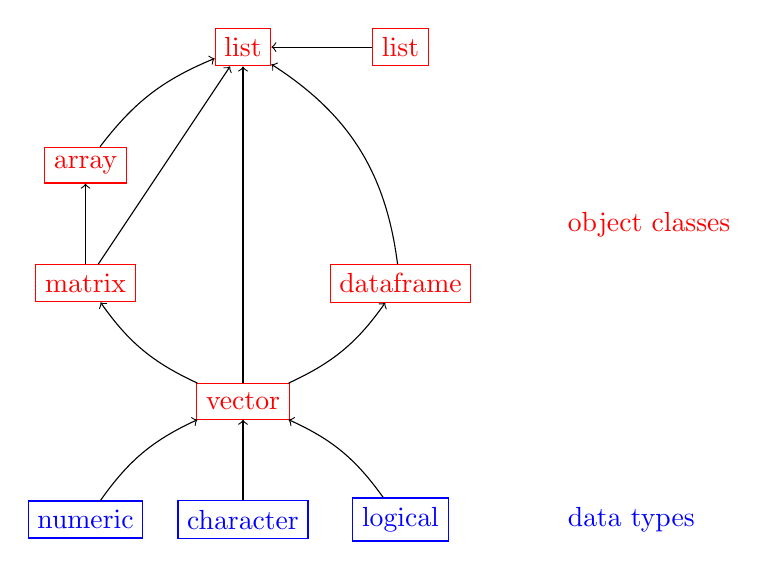
\begin{tikzpicture}
[class/.style={rectangle, draw=blue, blue}, type/.style={rectangle, draw=red, red}]

\node (num) at (0,0) [class] {numeric};
\node (char) at (2,0) [class] {character};
\node (logic) at (4,0) [class] {logical};
\node [blue,right] at (6,0) {data types};

\pause
\node (vec) at (2,1.5) [type] {vector}
  edge [<-, bend right = 15] (num)
  edge [<-] (char)
  edge [<-, bend left = 15] (logic);
\node [red,right] at (6,3.75) {object classes};
  
\pause
\node (mat) at (0,3) [type] {matrix}
  edge [<-, bend right = 15] (vec);
\node (dat) at (4,3) [type] {dataframe}
  edge [<-, bend left = 15] (vec);

\pause
\node (arr) at (0,4.5) [type] {array}
  edge [<-] (mat);

\pause
\node (list1) at (4,6) [type] {list};
\node (list) at (2,6) [type] {list}
  edge [<-] (vec)
  edge [<-, bend right = 15] (arr)
  edge [<-] (mat)
  edge [<-, bend left = 25] (dat)
  edge [<-] (list1);

\end{tikzpicture}
\end{center}
\end{frame}


\begin{frame}
\frametitle{exercises}
\begin{enumerate}
\item Create a vector of integers from 1 to 20.  
\item In one line of code, add 2, multiply by 5, take the square root, and then take the log of each element in the vector.
\item Create a vector of your 5 favorite cities.
\item Create a $3 \times 3$ matrix where each element of every column corresponds to the column number.
\item Convert this matrix into a dataframe.
\item Create a $3 \times 5 \times 2$ array of all 0s.
\item Create a list containing your array, your dataframe and your two vectors. 
\end{enumerate}
\end{frame}

\begin{frame}[fragile]
\frametitle{solutions}
\footnotesize
\begin{enumerate}
\item \red \footnotesize 
\begin{Schunk}
\begin{Sinput}
> ans.1 <- 1:20
\end{Sinput}
\end{Schunk}
\item \red \footnotesize
\begin{Schunk}
\begin{Sinput}
> ans.2 <- log(sqrt((ans.1 + 2) * 5))
\end{Sinput}
\end{Schunk}
\item \red \footnotesize
\begin{Schunk}
\begin{Sinput}
> ans.3 <- c("Los Angeles", "Las Vegas", "Hong Kong", "San Francisco", 
+     "Boston")
\end{Sinput}
\end{Schunk}
\item \red \footnotesize
\begin{Schunk}
\begin{Sinput}
> ans.4 <- matrix(c(1, 2, 3), ncol = 3, nrow = 3, byrow = T)
\end{Sinput}
\end{Schunk}
\item \red \footnotesize
\begin{Schunk}
\begin{Sinput}
> ans.5 <- as.data.frame(ans.4)
\end{Sinput}
\end{Schunk}
\item
\begin{Schunk}
\begin{Sinput}
> ans.6 <- array(0, dim = c(3, 5, 2))
\end{Sinput}
\end{Schunk}
\item 
\begin{Schunk}
\begin{Sinput}
> ans.7 <- list(ans.6, ans.5, ans.3, ans.2)
\end{Sinput}
\end{Schunk}
\end{enumerate}
\end{frame}

\section{Combining Objects}
\begin{frame}[fragile]
\frametitle{combining objects}
To combine vectors together or lists together, use \red{\tt c()}\black
\pause
\bigskip
\red
\begin{Schunk}
\begin{Sinput}
> vec1 <- c(4, 6, 9)
> vec2 <- 10:15
> comb.vec <- c(vec1, vec2)
> comb.vec
\end{Sinput}
\begin{Soutput}
[1]  4  6  9 10 11 12 13 14 15
\end{Soutput}
\end{Schunk}
\end{frame}

\begin{frame}[fragile]
To combine matrices or dataframes with other matrices, dataframes, or vectors, use \red{\tt cbind()} \black or \red{\tt rbind()}\black
\footnotesize
\pause
\bigskip
\red
\begin{Schunk}
\begin{Sinput}
> a.matrix <- matrix(0, nrow = 2, ncol = 3)
\end{Sinput}
\end{Schunk}
\pause
\begin{Schunk}
\begin{Sinput}
> rbind(a.matrix, 1:3)
\end{Sinput}
\begin{Soutput}
     [,1] [,2] [,3]
[1,]    0    0    0
[2,]    0    0    0
[3,]    1    2    3
\end{Soutput}
\end{Schunk}
\pause
\begin{Schunk}
\begin{Sinput}
> cbind(a.matrix, a.matrix)
\end{Sinput}
\begin{Soutput}
     [,1] [,2] [,3] [,4] [,5] [,6]
[1,]    0    0    0    0    0    0
[2,]    0    0    0    0    0    0
\end{Soutput}
\end{Schunk}
\normalsize
\black
\pause
\bigskip
Dimensions must match (think layered cake, not wedding cake).
\end{frame}

\section{Names}
\begin{frame}
\frametitle{names}
It's helpful to give names to elements or rows/columns within objects (i.e. variable names).\\
\pause
\bigskip
Use
\begin{itemize}
\item \red{\tt names()} \black for vectors, dataframes and lists
\pause
\item \red{\tt rownames()} \black and \red{\tt colnames()}\black for matrices and dataframes
\pause
\item \red{\tt dimnames()} \black for arrays
\end{itemize}
\end{frame}

\begin{frame}[fragile]
\red
\begin{Schunk}
\begin{Sinput}
> leaders <- c("Obama", "Brown", "Merkel")
> names(leaders) <- c("US", "UK", "Germany")
> leaders
\end{Sinput}
\begin{Soutput}
      US       UK  Germany 
 "Obama"  "Brown" "Merkel" 
\end{Soutput}
\end{Schunk}
\pause
\bigskip
\begin{Schunk}
\begin{Sinput}
> country.names <- names(leaders)
> country.names
\end{Sinput}
\begin{Soutput}
[1] "US"      "UK"      "Germany"
\end{Soutput}
\end{Schunk}
\end{frame}

\begin{frame}[fragile]
\red
\begin{Schunk}
\begin{Sinput}
> leader <- c("Obama", "Brown", "Merkel")
> year <- rep(2009, times = 3)
> dataset <- data.frame(cbind(leader, year))
\end{Sinput}
\end{Schunk}
\pause
\begin{Schunk}
\begin{Sinput}
> names(dataset) <- c("leader", "year")
> dataset
\end{Sinput}
\begin{Soutput}
  leader year
1  Obama 2009
2  Brown 2009
3 Merkel 2009
\end{Soutput}
\end{Schunk}
\pause
\bigskip
\black
\begin{itemize}
\item \red{\tt names()} \black and \red{\tt colnames()} \black are the same for dataframes only
\pause
\item must use \red{\tt colnames()}\black for matrices
\end{itemize}
\end{frame}

\section{Indexing and Subsetting}
\begin{frame}[fragile]
\frametitle{indexing}
Elements within objects are indexed using {\tt []} and {\tt [[]]}.
\pause
\bigskip
\begin{itemize}
\item vectors: {\tt [i]} for the ith element
\pause
\item matrices and dataframes: {\tt [i,j]} for the ith row, jth column
\pause
\item arrays: {\tt [i,j,k]} for the ith row, jth column, kth level
\pause
\item lists: [[i]] for the ith element
\end{itemize}
\end{frame}

\begin{frame}[fragile]
vectors:
\bigskip
\red
\footnotesize
\begin{Schunk}
\begin{Sinput}
> leaders
\end{Sinput}
\begin{Soutput}
      US       UK  Germany 
 "Obama"  "Brown" "Merkel" 
\end{Soutput}
\end{Schunk}
\pause
\bigskip
\begin{Schunk}
\begin{Sinput}
> leaders[2]
\end{Sinput}
\begin{Soutput}
     UK 
"Brown" 
\end{Soutput}
\end{Schunk}
\pause
\bigskip
\begin{Schunk}
\begin{Sinput}
> leaders[c(1, 3)]
\end{Sinput}
\begin{Soutput}
      US  Germany 
 "Obama" "Merkel" 
\end{Soutput}
\end{Schunk}
\end{frame}

\begin{frame}[fragile]
\red
\footnotesize
\begin{Schunk}
\begin{Sinput}
> leaders["US"]
\end{Sinput}
\begin{Soutput}
     US 
"Obama" 
\end{Soutput}
\end{Schunk}
\pause
\bigskip
\begin{Schunk}
\begin{Sinput}
> leaders[-3]
\end{Sinput}
\begin{Soutput}
     US      UK 
"Obama" "Brown" 
\end{Soutput}
\end{Schunk}
\end{frame}

\begin{frame}[fragile]
matrices and dataframes:
\bigskip
\red
\footnotesize
\begin{Schunk}
\begin{Sinput}
> dataset
\end{Sinput}
\begin{Soutput}
  leader year
1  Obama 2009
2  Brown 2009
3 Merkel 2009
\end{Soutput}
\end{Schunk}
\pause
\bigskip
\begin{Schunk}
\begin{Sinput}
> dataset[2, 1]
\end{Sinput}
\begin{Soutput}
[1] Brown
Levels: Brown Merkel Obama
\end{Soutput}
\end{Schunk}
\pause
\bigskip
\begin{Schunk}
\begin{Sinput}
> dataset[2, ]
\end{Sinput}
\begin{Soutput}
  leader year
2  Brown 2009
\end{Soutput}
\end{Schunk}
\end{frame}

\begin{frame}[fragile]
\footnotesize
\red
\begin{Schunk}
\begin{Sinput}
> dataset[, "year"]
\end{Sinput}
\begin{Soutput}
[1] 2009 2009 2009
Levels: 2009
\end{Soutput}
\end{Schunk}
\pause
\bigskip
\begin{Schunk}
\begin{Sinput}
> dataset[, -1]
\end{Sinput}
\begin{Soutput}
[1] 2009 2009 2009
Levels: 2009
\end{Soutput}
\end{Schunk}
\pause
\bigskip
\black
\normalsize
for datasets:
\red
\footnotesize
\pause
\bigskip
\begin{Schunk}
\begin{Sinput}
> dataset$leader
\end{Sinput}
\begin{Soutput}
[1] Obama  Brown  Merkel
Levels: Brown Merkel Obama
\end{Soutput}
\end{Schunk}
\end{frame}

\begin{frame}[fragile]
lists:
\bigskip
\red
\footnotesize
\begin{Schunk}
\begin{Sinput}
> my.list <- list(mat = a.matrix, vec = leaders)
> my.list
\end{Sinput}
\begin{Soutput}
$mat
     [,1] [,2] [,3]
[1,]    0    0    0
[2,]    0    0    0

$vec
      US       UK  Germany 
 "Obama"  "Brown" "Merkel" 
\end{Soutput}
\end{Schunk}
\pause
\begin{Schunk}
\begin{Sinput}
> names(my.list)
\end{Sinput}
\begin{Soutput}
[1] "mat" "vec"
\end{Soutput}
\end{Schunk}
\end{frame}

\begin{frame}[fragile]
\red
\footnotesize
\begin{Schunk}
\begin{Sinput}
> my.list[[2]]
\end{Sinput}
\begin{Soutput}
      US       UK  Germany 
 "Obama"  "Brown" "Merkel" 
\end{Soutput}
\end{Schunk}
\pause
\bigskip
\begin{Schunk}
\begin{Sinput}
> my.list[[2]][2]
\end{Sinput}
\begin{Soutput}
     UK 
"Brown" 
\end{Soutput}
\end{Schunk}
\pause
\bigskip
\begin{Schunk}
\begin{Sinput}
> my.list$mat
\end{Sinput}
\begin{Soutput}
     [,1] [,2] [,3]
[1,]    0    0    0
[2,]    0    0    0
\end{Soutput}
\end{Schunk}
\end{frame}

\section{Editing and Subsetting Objects}
\begin{frame}[fragile]
\frametitle{editing objects}
Now that we know indexing, editing and subsetting objects is trivial.\\
\pause
\bigskip
For example, we can add to an object (such as adding a variable to a dataset):
\pause
\bigskip
\red
\footnotesize
\begin{Schunk}
\begin{Sinput}
> dataset$europe <- c(0, 0, 1)
> dataset
\end{Sinput}
\begin{Soutput}
  leader year europe
1  Obama 2009      0
2  Brown 2009      0
3 Merkel 2009      1
\end{Soutput}
\end{Schunk}
\end{frame}

\begin{frame}[fragile]
or edit an object:
\red
\pause
\bigskip
\footnotesize
\begin{Schunk}
\begin{Sinput}
> dataset[2, "europe"] <- 1
> dataset
\end{Sinput}
\begin{Soutput}
  leader year europe
1  Obama 2009      0
2  Brown 2009      1
3 Merkel 2009      1
\end{Soutput}
\end{Schunk}
\end{frame}

\begin{frame}[fragile]
\frametitle{subsetting objects}
with logical statements:
\bigskip
\pause
\red
\footnotesize
\begin{Schunk}
\begin{Sinput}
> dataset$europe == 1
\end{Sinput}
\begin{Soutput}
[1] FALSE  TRUE  TRUE
\end{Soutput}
\end{Schunk}
\pause
\begin{Schunk}
\begin{Sinput}
> dataset[dataset$europe == 1, ]
\end{Sinput}
\begin{Soutput}
  leader year europe
2  Brown 2009      1
3 Merkel 2009      1
\end{Soutput}
\end{Schunk}
\normalsize
\pause
\bigskip
\black
{\tt $==$, \pause $!=$, \pause $>$, \pause $<$, \pause $>=$, \pause $<=$\\
$\&$, \pause $\mid$, \pause \%in\% }
\end{frame}

\section{The R Environment}
\begin{frame}[fragile]
\frametitle{the R environment}
Any objects you create will be stored in the R environment. \\
\pause
\bigskip
To see all the objects in your environment:
\pause
\red
\footnotesize
\begin{Schunk}
\begin{Sinput}
> ls()
\end{Sinput}
\begin{Soutput}
 [1] "a.dataframe"    "a.list"         "a.matrix"       "a.vec"         
 [5] "add.vec"        "all.fours"      "an.array"       "ans.1"         
 [9] "ans.2"          "ans.3"          "ans.4"          "ans.5"         
[13] "ans.6"          "ans.7"          "beta.func"      "beta.hat"      
[17] "comb.vec"       "country.names"  "data.samp"      "dataset"       
[21] "diff.func"      "empty.vector"   "first.draws"    "geomean.func"  
[25] "i"              "j"              "just.trade"     "leader"        
[29] "leaders"        "logical.vec"    "macro"          "macro.subset"  
[33] "means"          "medians"        "mixed.vec"      "mixed.vec2"    
[37] "my.list"        "my.name"        "my.sum"         "new.data"      
[41] "new.macro"      "num.vec"        "one.to.five"    "one.to.ten"    
[45] "PErisk"         "poli.sci"       "population"     "president"     
[49] "pull.out.trade" "quants"         "random.numbers" "results"       
[53] "results.vec"    "row.numbers"    "row.samp"       "samp"          
[57] "samp.data"      "samp.w.probs"   "samp.w.rep"     "samp.wo.rep"   
[61] "sds"            "second.draws"   "tally"          "test.mat"      
[65] "test.matrix"    "test.vec"       "three"          "triangle.func" 
[69] "trim.func"      "trimmed.1"      "trimmed.25"     "two.func"      
[73] "two.to.five"    "variables"      "vec1"           "vec2"          
[77] "vector"         "X"              "xy.func"        "y"             
[81] "year"          
\end{Soutput}
\end{Schunk}
\normalsize
\black
\pause
\bigskip
To remove an object:
\pause
\red
\footnotesize
\begin{Schunk}
\begin{Sinput}
> rm(vec1)
\end{Sinput}
\end{Schunk}
\end{frame}

\section{Packages}
\begin{frame}
\frametitle{packages}
To use packages, you need to install them (do this once) and load them (every time you open R).\\
\pause
\bigskip
To install a package named {\tt foo}:
\pause
\begin{enumerate}
\item type \red{\tt install.packages("foo")}\black
\pause
\item choose a CRAN repository
\end{enumerate}
\bigskip
\pause
To load a package named {\tt foo}:
\pause
\begin{enumerate}
\item type \red{\tt library(foo)}\black
\end{enumerate}
\end{frame}

\section{Loading Data}
\begin{frame}
\frametitle{loading datasets}
Suppose you want to load the {\tt foo} dataset. \\
\pause
\bigskip
If the dataset is in
\begin{itemize}
\item an existing R package, load the package and type \red{\tt data(foo)}\black
\pause
\item .RData format, type \red{\tt load(foo)}\black
\pause
\item .txt or other text formats, type \red{\tt read.table("foo.txt")}\black
\pause
\item .csv format, type \red{\tt read.csv("foo.csv")}\black
\pause
\item .dta (Stata) format, load the {\tt foreign} library and type \red{\tt read.dta("foo.dta")}\black
\end{itemize}
\pause
\bigskip
To save objects into these formats, use the equivalent \red {\tt write.table()}\black, \red{\tt write.csv()}\black, etc. commands. 
\end{frame}

\section{Working Directory}
\begin{frame}
\frametitle{working directory}
When loading or saving a dataset or object, R will look in the current working directory.\\
\pause
\bigskip
If your working directory is not where the file is at, R will not find it, so make sure you change the working directory.
\pause
\bigskip
\begin{itemize}
\item to change to the {\tt foo} working directory, use \red {\tt setwd("foo")} \black
\pause
\item to see the current working directory, type \red {\tt getwd()} \black
\end{itemize}
\end{frame}

\begin{frame}
\frametitle{exercises}
\begin{enumerate}
\item Load the {\tt macro} dataset from the {\tt Zelig} package.
\item Change the name of the ``year" variable in the dataset to ``date".
\item Add a column of just 1s to the left of the dataset.
\item Create a vector with just the ``trade" variable from the dataset.
\item Create a new dataset with all the observations where "gdp" is greater than 3.25 and ``unem" is less than 5.
\item Write this new smaller dataset as a separate file into your working directory in any format (i.e. .csv, .dta, .txt)
\item Store the large dataset, the ``trade" vector, and the new smaller dataset in a list with appropriate names.  Then extract the ``trade" vector from the list.
\end{enumerate}
\end{frame}

\begin{frame}[fragile]
\frametitle{solutions}
\begin{enumerate}
\red
\footnotesize
\item 
\begin{Schunk}
\begin{Sinput}
> library(Zelig)
> data(macro)
\end{Sinput}
\end{Schunk}
\item 
\begin{Schunk}
\begin{Sinput}
> names(macro)[2] <- "date"
\end{Sinput}
\end{Schunk}
\item
\begin{Schunk}
\begin{Sinput}
> new.macro <- cbind(1, macro)
\end{Sinput}
\end{Schunk}
\item 
\begin{Schunk}
\begin{Sinput}
> just.trade <- macro$trade
\end{Sinput}
\end{Schunk}
\item
\begin{Schunk}
\begin{Sinput}
> macro.subset <- macro[macro$gdp > 3.25 & macro$unem < 5, 
+     ]
\end{Sinput}
\end{Schunk}
\item
\begin{Schunk}
\begin{Sinput}
> write.csv(macro.subset, file = "macrosubset.csv")
\end{Sinput}
\end{Schunk}
\item 
\begin{Schunk}
\begin{Sinput}
> my.list <- list(large = new.macro, small = macro.subset, 
+     trade = just.trade)
> pull.out.trade <- my.list$trade
\end{Sinput}
\end{Schunk}
\end{enumerate}
\end{frame}

\section{Analyzing Vectors}
\begin{frame}
\frametitle{analyzing vectors}
\pause
\begin{itemize}
\red
\item {\tt mean()}
\item {\tt median()}
\item {\tt sd()}
\item {\tt var()}
\item {\tt cor()}
\item {\tt cov()}
\item {\tt quantile()}
\item {\tt max()}
\item {\tt min()}
\end{itemize}
\end{frame}

\begin{frame}
\frametitle{other vector functions}
\pause
\begin{itemize}
\red
\item {\tt sum()}
\item {\tt prod()}
\item {\tt length()}
\item {\tt table()}
\item {\tt unique()}
\item {\tt sort()}
\item {\tt order()}
\item {\tt which()} \black with logical statements
\end{itemize}
\end{frame}

\section{Analyzing Dataframes and Matrices}
\begin{frame}
\frametitle{analyzing dataframes and matrices}
\pause
\begin{itemize}
\red
\item {\tt head()}
\item {\tt tail()}
\item {\tt nrow()}
\item {\tt ncol()}
\item {\tt summary()}
\item {\tt colMeans()}
\item {\tt rowMeans()}
\item {\tt colSums()}
\item {\tt rowSums()}
\item {\tt View()}
\item {\tt edit()}
\end{itemize}
\end{frame}

\begin{frame}
\frametitle{exercises}
\pause
\begin{enumerate}
\item Reload the {\tt macro} dataset from {\tt Zelig}.  Find the mean, median, standard deviation, and 20th and 80th percent quantiles of the unemployment variable.
\item How many observations are there in this dataset?
\item What's the correlation between trade and gdp?
\item Which country-year observation had the highest unemployment rate in the dataset?
\item Which country had the most number of years where gdp > 5?
\end{enumerate}
\end{frame}

\begin{frame}[fragile]
\frametitle{solutions}
\begin{enumerate}
\red
\footnotesize
\item
\begin{Schunk}
\begin{Sinput}
> data(macro)
> mean(macro$unem)
\end{Sinput}
\begin{Soutput}
[1] 4.993873
\end{Soutput}
\begin{Sinput}
> median(macro$unem)
\end{Sinput}
\begin{Soutput}
[1] 4.5
\end{Soutput}
\begin{Sinput}
> sd(macro$unem)
\end{Sinput}
\begin{Soutput}
[1] 3.240486
\end{Soutput}
\begin{Sinput}
> quantile(macro$unem, probs = c(0.2, 0.8))
\end{Sinput}
\begin{Soutput}
     20%      80% 
1.880000 8.105564 
\end{Soutput}
\end{Schunk}
\item
\begin{Schunk}
\begin{Sinput}
> nrow(macro)
\end{Sinput}
\begin{Soutput}
[1] 350
\end{Soutput}
\end{Schunk}
\end{enumerate}
\end{frame}

\begin{frame}[fragile]
\begin{enumerate}
\red
\footnotesize
\item[3.]
\begin{Schunk}
\begin{Sinput}
> cor(macro$trade, macro$gdp)
\end{Sinput}
\begin{Soutput}
[1] -0.220669
\end{Soutput}
\end{Schunk}
\item[4.]
\begin{Schunk}
\begin{Sinput}
> macro[macro$unem == max(macro$unem), c("country", "year")]
\end{Sinput}
\begin{Soutput}
    country year
119 Belgium 1984
\end{Soutput}
\end{Schunk}
\item[5.]
\begin{Schunk}
\begin{Sinput}
> tally <- table(macro$country[macro$gdp > 5])
> names(tally)[tally == max(tally)]
\end{Sinput}
\begin{Soutput}
[1] "Japan"
\end{Soutput}
\end{Schunk}
\end{enumerate}
\end{frame}

\section{Functions}
\begin{frame}
\frametitle{functions}
One last object class that we have yet to mention are {\bf functions}.\\
\bigskip
\pause
Basically everything in R is performing a function on an object.\\
\pause
\bigskip
Recall a function in math:
\pause
\begin{center}
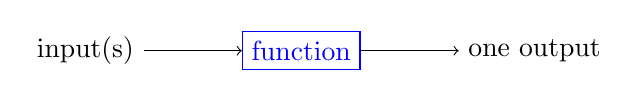
\begin{tikzpicture}
[func/.style={rectangle, draw=blue, blue}, type/.style={rectangle, draw=red, red}]

\node (inp) [black,left] at (0,0) {input(s)};
\node (func) at (2,0) [func] {function}
 edge[<-] (inp);
\node [black,right] at (4,0) {one output}
 edge[<-](func);

\end{tikzpicture}
\end{center}
\pause
\bigskip
Functions in R:
\pause
\begin{center}
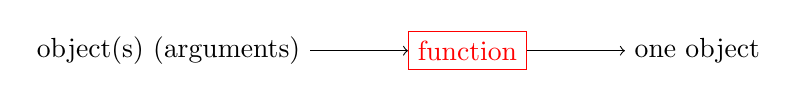
\begin{tikzpicture}
[func/.style={rectangle, draw=red, red}, type/.style={rectangle, draw=red, red}]

\node (inp) [black,left] at (0,0) {object(s) (arguments)};
\node (func) at (2,0) [func] {function}
 edge[<-] (inp);
\node [black,right] at (4,0) {one object}
 edge[<-](func);

\end{tikzpicture}
\end{center}
\pause
\bigskip
Up to now, we've used many canned functions, but we will also need to write our own functions.
\end{frame}

\begin{frame}[fragile]
$f(x,y) = x^2 + y^2$
\pause
\bigskip
\red
\footnotesize
\begin{Schunk}
\begin{Sinput}
> xy.func <- function(x, y) {
+     f.xy <- x^2 + y^2
+     return(f.xy)
+ }
\end{Sinput}
\end{Schunk}
\pause
\begin{Schunk}
\begin{Sinput}
> xy.func(x = 3, y = 4)
\end{Sinput}
\begin{Soutput}
[1] 25
\end{Soutput}
\end{Schunk}
\pause
\black
\normalsize
or
\pause
\footnotesize
\red
\begin{Schunk}
\begin{Sinput}
> xy.func <- function(vec) {
+     x <- vec[1]
+     y <- vec[2]
+     f.xy <- x^2 + y^2
+     return(f.xy)
+ }
\end{Sinput}
\end{Schunk}
\pause
\begin{Schunk}
\begin{Sinput}
> xy.func(vec = c(3, 4))
\end{Sinput}
\begin{Soutput}
[1] 25
\end{Soutput}
\end{Schunk}
\end{frame}

\begin{frame}[fragile]
a function that deletes the first $p$ percent of observations from a dataframe
\pause
\red
\footnotesize
\bigskip
\begin{Schunk}
\begin{Sinput}
> trim.func <- function(x, p = .1){
+   n <- nrow(x)  #number of observations
+   trim.number <- round(p*n)  #number to delete (rounded)
+   trimmed.data <- x[-c(1:trim.number),] #delete from top
+   return(trimmed.data)
+ }
\end{Sinput}
\end{Schunk}
\pause
\bigskip
\begin{Schunk}
\begin{Sinput}
> data(macro)
> trimmed.1 <- trim.func(x = macro)
> trimmed.25 <- trim.func(x = macro, p = 0.25)
\end{Sinput}
\end{Schunk}
\end{frame}

\begin{frame}
\frametitle{looking for help}
Suppose you want help for a certain function or dataset in R (i.e. what are the arguments of the function, what does the function do, etc.).\\ 
\bigskip
\pause To look for help with a function called {\tt foo()}, you can type in one of the following:
\pause
\begin{itemize}
\red
\item {\tt ?foo}
\item {\tt help("foo")}
\end{itemize}
\pause
\bigskip
To search for a function by keyword, type in {\tt \red help.search("keyword")}.
\end{frame}

\begin{frame}
\frametitle{how to read a help file}
\pause
Most help files follow an approximate format:
\bigskip
\begin{itemize}
\item description: briefly describes what the function does
\item usage: the syntax for the function as well as arguments and its defaults
\item arguments: more specific details about what goes in the arguments
\item details: more elaborate description of what the function does
\item value: quantities that you can extract from the function (the output)
\item more notes and references
\item similar functions in R
\item example code you can run
\end{itemize}
\end{frame}


\begin{frame}
\frametitle{exercises}
\begin{enumerate}
\item Write a function that calculates the geometric mean of a vector of numbers:
\begin{eqnarray*}
G =  \left( \prod^n_{i=1} X_n \right) ^ {\frac{1}{n}}
\end{eqnarray*}
\item Write a function that takes in a matrix, finds the column of the matrix that has the smallest sum, and then produces a list with the mean, median, standard deviation, and the 25th and 75th percentiles of that column.
\end{enumerate}
\end{frame}

\begin{frame}[fragile]
\frametitle{solutions}
\begin{enumerate}
\red
\footnotesize
\item
\begin{Schunk}
\begin{Sinput}
> geomean.func <- function(x){  ## x is a vector 
+   G <- prod(x)^(1/length(x))
+   return(G)
+ }
> test.vec <- c(1,2,3)
> geomean.func(test.vec)
\end{Sinput}
\begin{Soutput}
[1] 1.817121
\end{Soutput}
\end{Schunk}
\end{enumerate}
\end{frame}

\begin{frame}[fragile]
\begin{enumerate}
\red
\footnotesize
\item[2.]
\begin{Schunk}
\begin{Sinput}
> two.func <- function(x){  ## x is a matrix
+   which.col <- which(colSums(x) == min(colSums(x)))
+   column <- x[,which.col] ## extract column
+   output <- list(mean = mean(column), median = median(column), 
+   sd=sd(column), percentiles=quantile(column, probs=c(.25,.75)))
+   return(output)
+ }
> random.numbers <- sample(1:100, 81)
> test.mat <- matrix(random.numbers, nrow = 9, ncol = 9)
> two.func(test.mat)
\end{Sinput}
\begin{Soutput}
$mean
[1] 43.22222

$median
[1] 39

$sd
[1] 31.29208

$percentiles
25% 75% 
 16  68 
\end{Soutput}
\end{Schunk}
\end{enumerate}
\end{frame}

\section{The Apply Function}
\begin{frame}
\frametitle{apply()}
The {\tt \red apply()} function takes a function and applies it on each row or column of a matrix, dataframe, or array.
\bigskip
\pause
\begin{itemize}
\item the MARGIN argument gets 1 for row and 2 for column
\pause
\item typically, though not necessarily, the function to be applied is a function that takes in vectors
\pause
\item any extra arguments to the function being applied can be defined after the FUN argument
\pause
\item {\tt \red lapply()}, {\tt \red sapply()}, and {\tt \red tapply()} are functions that do similar things
\end{itemize}
\end{frame}

\begin{frame}[fragile]
take the median of every row
\bigskip
\red
\footnotesize
\begin{Schunk}
\begin{Sinput}
> test.matrix <- matrix(1:9, ncol = 3, nrow = 3)
> test.matrix
\end{Sinput}
\begin{Soutput}
     [,1] [,2] [,3]
[1,]    1    4    7
[2,]    2    5    8
[3,]    3    6    9
\end{Soutput}
\begin{Sinput}
> medians <- apply(test.matrix, MARGIN = 1, FUN = median)
> medians
\end{Sinput}
\begin{Soutput}
[1] 4 5 6
\end{Soutput}
\end{Schunk}
\end{frame}

\begin{frame}[fragile]
take the geometric mean of every column
\bigskip
\red
\footnotesize
\begin{Schunk}
\begin{Sinput}
> geomean.func <- function(x) {
+     G <- prod(x)^(1/length(x))
+     return(G)
+ }
> test.matrix <- matrix(11:19, ncol = 3, nrow = 3)
> apply(test.matrix, MARGIN = 2, FUN = geomean.func)
\end{Sinput}
\begin{Soutput}
[1] 11.97216 14.97774 17.98146
\end{Soutput}
\end{Schunk}
\end{frame}

\begin{frame}[fragile]
find the 25th and 75th quantile of every column of {\tt macro}
\bigskip
\red
\footnotesize
\begin{Schunk}
\begin{Sinput}
> library(Zelig)
> data(macro)
> ## take out the first two columns, which are country and year
> apply(macro[,-c(1,2)], MARGIN=2, FUN=quantile, probs=c(.25,.75))
\end{Sinput}
\begin{Soutput}
         gdp     unem capmob    trade
25% 1.877098 2.099248     -1 41.41939
75% 4.700000 7.300000      0 71.84709
\end{Soutput}
\begin{Sinput}
> summary(macro[,-c(1,2)])
\end{Sinput}
\begin{Soutput}
      gdp              unem             capmob            trade        
 Min.   :-4.300   Min.   : 0.6848   Min.   :-4.0000   Min.   :  9.623  
 1st Qu.: 1.877   1st Qu.: 2.0992   1st Qu.:-1.0000   1st Qu.: 41.419  
 Median : 3.200   Median : 4.5000   Median :-1.0000   Median : 52.624  
 Mean   : 3.254   Mean   : 4.9939   Mean   :-0.8914   Mean   : 57.076  
 3rd Qu.: 4.700   3rd Qu.: 7.3000   3rd Qu.: 0.0000   3rd Qu.: 71.847  
 Max.   :12.800   Max.   :13.0000   Max.   : 0.0000   Max.   :146.020  
\end{Soutput}
\end{Schunk}
\end{frame}

\section{Sampling}
\begin{frame}[fragile]
\frametitle{sampling}
Sampling from a vector can be done with the {\tt \red sample()} function.
\bigskip
\pause
\red
\footnotesize
\begin{Schunk}
\begin{Sinput}
> population <- c(1, 2, 3, 4, 5)
> samp.w.rep <- sample(population, size = 3, replace = T)
> samp.w.rep
\end{Sinput}
\begin{Soutput}
[1] 5 2 3
\end{Soutput}
\end{Schunk}
\pause
\medskip
\begin{Schunk}
\begin{Sinput}
> samp.wo.rep <- sample(population, size = 3, replace = F)
> samp.wo.rep
\end{Sinput}
\begin{Soutput}
[1] 5 3 2
\end{Soutput}
\end{Schunk}
\pause
\medskip
\begin{Schunk}
\begin{Sinput}
> samp.w.probs <- sample(population, size = 3, replace = T, 
+     prob = c(0.8, 0.05, 0.05, 0.05, 0.05))
> samp.w.probs
\end{Sinput}
\begin{Soutput}
[1] 1 1 1
\end{Soutput}
\end{Schunk}
\end{frame}

\section{For Loops}
\begin{frame}
\frametitle{for loops}
Use a {\tt \red for} loop to repeat some code over and over again.
\pause
\bigskip
\begin{itemize}
\item typically good for things like sampling multiple times
\pause
\item very computationally intensive, so use as last resort
\pause
\item many things can be done using {\tt \red apply()} instead
\end{itemize}
\end{frame}

\begin{frame}[fragile]
\red
\footnotesize
\begin{Schunk}
\begin{Sinput}
> vector <- c(1, 5, 8, 3, 5, 2, 97, 430)
> for (i in vector) {
+     print(i)
+ }
\end{Sinput}
\begin{Soutput}
[1] 1
[1] 5
[1] 8
[1] 3
[1] 5
[1] 2
[1] 97
[1] 430
\end{Soutput}
\end{Schunk}
\bigskip \pause
\black \normalsize
\begin{itemize}
\item each time runs through everything between {\tt \red \{ \}}
\item each time, "i" is defined to be an element of the vector (first time "i" is the first element, second time "i" is the second element, etc.)
\item loop runs as many times as the length of the vector
\end{itemize}
\end{frame}

\begin{frame}[fragile]
a loop that adds 5 to each of the loop indices and stores the output in a vector
\bigskip
\red
\footnotesize
\begin{Schunk}
\begin{Sinput}
> add.vec <- c()
> for (j in 1:10){
+   ## add 5 to j and put in jth slot of the add.vec vector
+   add.vec[j] <- j + 5 
+ }
> add.vec
\end{Sinput}
\begin{Soutput}
 [1]  6  7  8  9 10 11 12 13 14 15
\end{Soutput}
\end{Schunk}
\end{frame}

\section{Conditional Statements}
\begin{frame}[fragile]
\frametitle{conditional statements}
\pause
Conditional statements may come in handy when manipulating data:
\pause
\bigskip
\begin{itemize}
\item {\tt \red if()\{\}} and {\tt \red else\{\}}
\item {\tt \red ifelse()}
\end{itemize}
\end{frame}

\begin{frame}[fragile]
$$
f(x) = \left\lbrace \begin{array}{ll} 8x & \mathrm{if} \;
0 \le x < 0.25 \\
\frac{8}{3} - \frac{8}{3} x & \mathrm{if} \; 0.25 \le x \le 1 \\
0 & \mathrm{otherwise} \end{array} \right. 
$$
\bigskip
\pause
\red
\footnotesize
\begin{Schunk}
\begin{Sinput}
> triangle.func <- function(x) {
+     if (x >= 0 & x < 0.25) {
+         out <- 8 * x
+     }
+     else if (x >= 0.25 & x <= 1) {
+         out <- 8/3 - 8 * x/3
+     }
+     else {
+         out <- 0
+     }
+     return(out)
+ }
\end{Sinput}
\end{Schunk}
\end{frame}

\begin{frame}[fragile]
Create a new variable in {\tt macro} for whether the observation is before or after 1980.
\bigskip
\pause
\red
\footnotesize
\begin{Schunk}
\begin{Sinput}
> macro$pre1980 <- ifelse(macro$year < 1980, 1, 0)
\end{Sinput}
\end{Schunk}
\bigskip
\pause
\black
\normalsize
Everything done using {\tt \red ifelse()} can be done using {\tt \red if} and {\tt \red else}, but the code may be less efficient.
\end{frame}

\begin{frame}[fragile]
\frametitle{exercises}
You will need the {\tt macro} dataset from {\tt Zelig}.
\bigskip
\begin{enumerate}
\item Write a function that takes in a vector and outputs the maximum of the vector minus the minimum of the vector.
\item Apply the function you wrote above to columns of {\tt macro}, omitting the country and year variables.
\end{enumerate}
\end{frame}

\begin{frame}[fragile]
\begin{enumerate}
\item[3.] Omit the country and year variables from {\tt macro}.  Take a sample of 350 observations from the dataset with replacement (hint: sample row numbers).  Take the mean of each column in your sample.  Do this 1000 times and store your results in a $1000 \times 4$ matrix.
\item[4.] Take a sample of size 200 from {\tt macro\$trade} without replacement.  If the absolute value ({\tt \red abs()}) of the difference between the max and the min of this sample is greater than 3 times the standard deviation of {\tt macro\$trade}, then take the median of the sample.  Otherwise take the mean.  Do this 1000 times and store the results of your 1000 iterations in a vector.
\item[5.] Create a new variable in {\tt macro} called "rich" where for each observation, the variable takes on a value of 1 if its gdp is greater than the mean gdp and 0 otherwise.
\end{enumerate}
\end{frame}

\begin{frame}[fragile]
\frametitle{solutions}
\begin{enumerate}
\red
\footnotesize
\item 
\begin{Schunk}
\begin{Sinput}
> diff.func <- function(x){ ## x is a vector
+   out <- max(x) - min(x)
+   return(out)
+ }
\end{Sinput}
\end{Schunk}
\medskip
\item 
\begin{Schunk}
\begin{Sinput}
> data(macro)
> apply(macro[, -c(1, 2)], MARGIN = 2, FUN = diff.func)
\end{Sinput}
\begin{Soutput}
      gdp      unem    capmob     trade 
 17.10000  12.31522   4.00000 136.39729 
\end{Soutput}
\end{Schunk}
\medskip
\item 
\begin{Schunk}
\begin{Sinput}
> new.macro <- macro[,-c(1,2)]
> results <- matrix(NA, nrow = 1000, ncol = 4) # results matrix
> for (i in 1:1000){
+   row.samp <- sample(c(1:nrow(new.macro)), size = 350, 
+   replace = T) 
+   data.samp <- new.macro[row.samp,]
+   results[i,] <- colMeans(data.samp)
+ }
\end{Sinput}
\end{Schunk}
\end{enumerate}
\end{frame}

\begin{frame}[fragile]
\begin{enumerate}
\red
\footnotesize
\item [4.]
\begin{Schunk}
\begin{Sinput}
> results.vec <- c()
> for (i in 1:1000) {
+     samp <- sample(macro$trade, size = 200, replace = F)
+     if (abs(max(samp) - min(samp)) > 3 * sd(macro$trade)) {
+         results.vec[i] <- median(samp)
+     }
+     else {
+         results.vec[i] <- mean(samp)
+     }
+ }
\end{Sinput}
\end{Schunk}
\medskip
\item [5.]
\begin{Schunk}
\begin{Sinput}
> macro$rich <- ifelse(macro$gdp > mean(macro$gdp), 1, 0)
\end{Sinput}
\end{Schunk}
\end{enumerate}

\end{frame}

\section{Plotting}
\begin{frame}[fragile]
\frametitle{plots}
\begin{itemize}
\item specialized plots: {\tt \red hist()}, {\tt \red barplot()}, etc.
\pause
\item general plot command for lines, points, etc.: {\tt \red plot()}
\pause
\item many options using {\tt \red par()} before {\tt \red plot()} 
\pause
\item add a legend using {\tt \red legend()}
\pause
\item add points with {\tt \red points()}
\end{itemize}
\end{frame}

\begin{frame}[fragile]
scatterplot:
\red
\footnotesize
\medskip
\begin{Schunk}
\begin{Sinput}
> plot(x = macro$trade, y = macro$gdp, xlab = "Trade", ylab = "GDP", 
+     main = "Scatterplot of Trade and GDP")
\end{Sinput}
\end{Schunk}
\begin{figure}
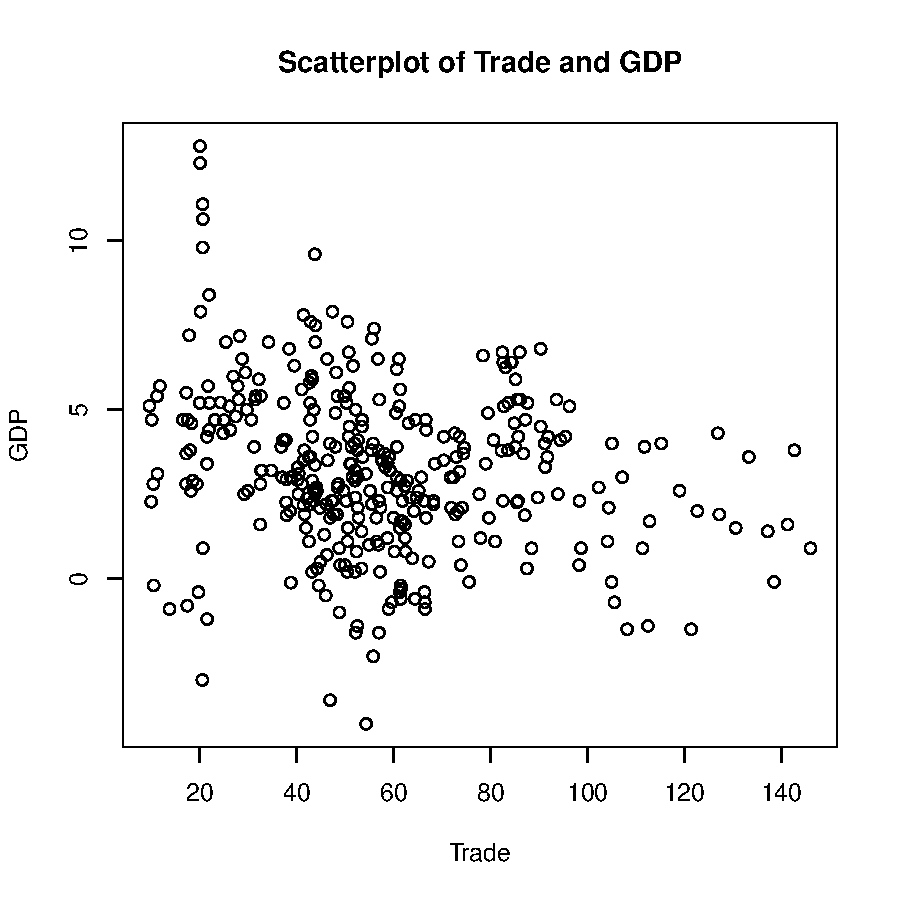
\includegraphics[width=2in, height=2in]{rslides-plot1.pdf}
\end{figure}
\end{frame}

\begin{frame}[fragile]
density plot:
\red
\footnotesize
\medskip
\begin{Schunk}
\begin{Sinput}
> plot(density(macro$trade), main = "Density Plot of Trade")
\end{Sinput}
\end{Schunk}
\begin{figure}
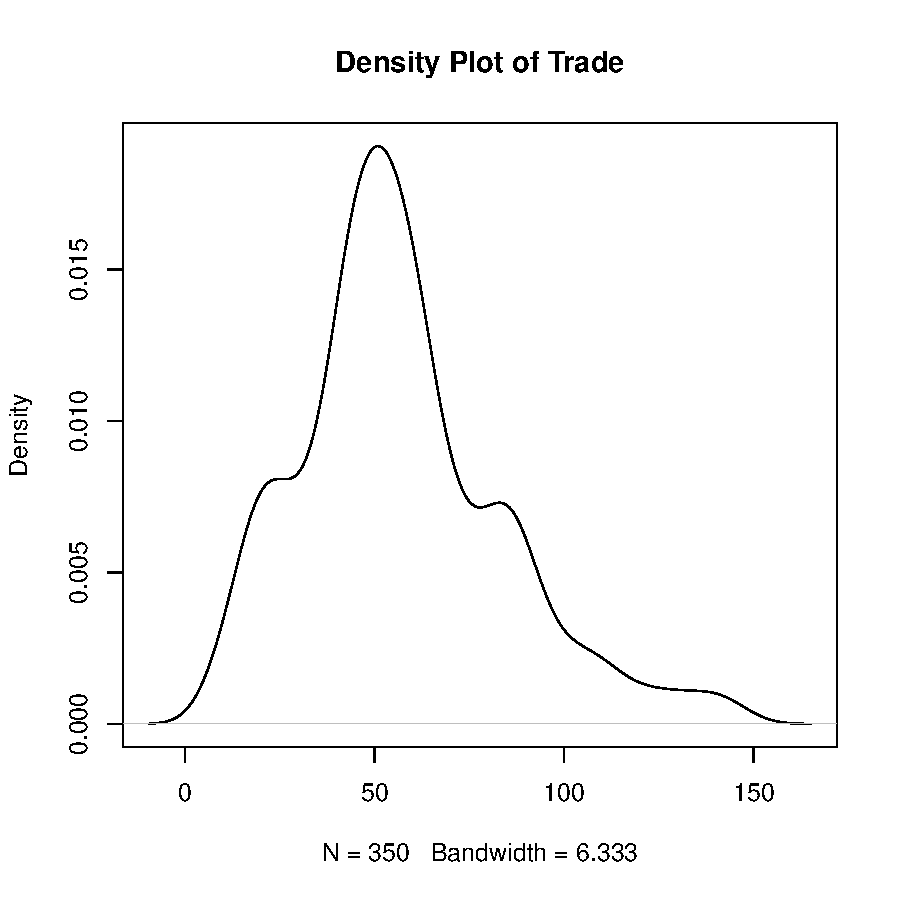
\includegraphics[width=2in, height=2in]{rslides-plot2.pdf}
\end{figure}
\end{frame}

\begin{frame}[fragile]
multiple line plots in one (with legend):
\red
\footnotesize
\medskip
\begin{Schunk}
\begin{Sinput}
> plot(density(macro$gdp), main = "Density Plots")
> lines(density(macro$unem), col = "red", lty = "dashed")
> legend(x = "topright", legend = c("GDP", "Unemployment"), 
+     lty = c("solid", "dashed"), col = c("black", "red"))
\end{Sinput}
\end{Schunk}
\begin{figure}
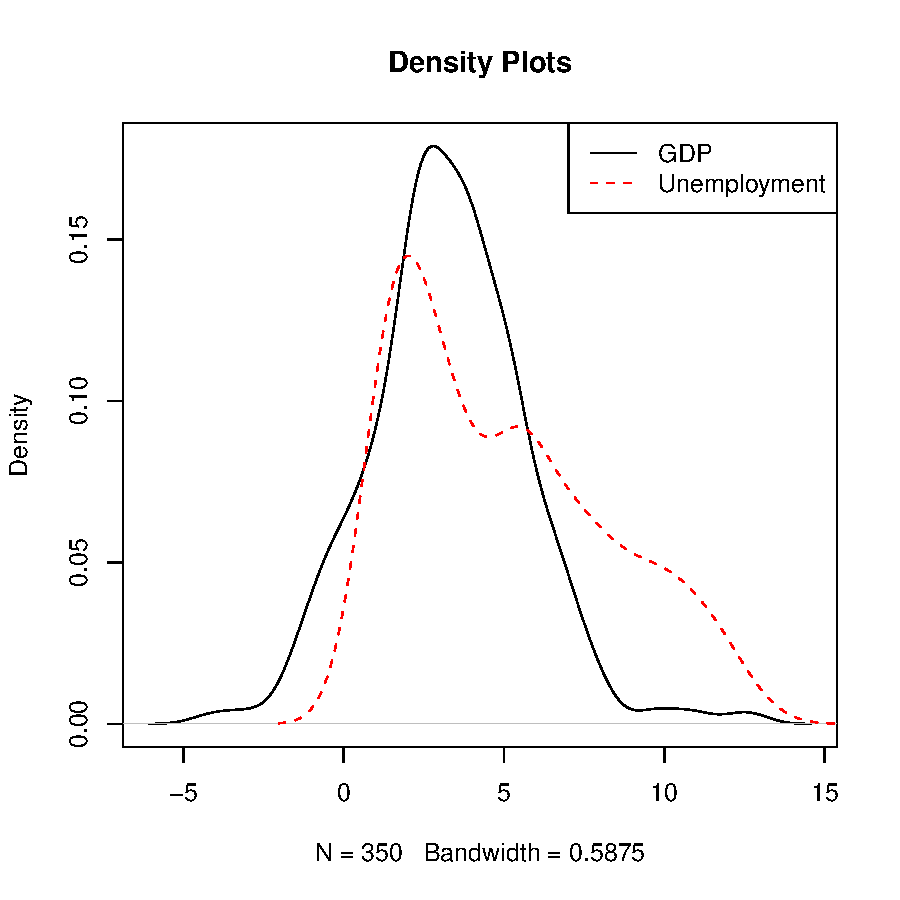
\includegraphics[width=2in, height=2in]{rslides-plot3.pdf}
\end{figure}
\end{frame}

\begin{frame}[fragile]
add a straight line with {\tt \red abline()}:
\red
\footnotesize
\medskip
\begin{Schunk}
\begin{Sinput}
> plot(x = macro$trade, y = macro$gdp, xlab = "Trade", ylab = "GDP", 
+     main = "Scatterplot of Trade and GDP")
> abline(a = 0, b = 0.1, col = "red")
> abline(v = 80, col = "blue")
\end{Sinput}
\end{Schunk}
\begin{figure}
\includegraphics[width=2in, height=2in]{rslides-plot4.pdf}
\end{figure}
\end{frame}

\begin{frame}[fragile]
multiple plots with {\tt \red par()} options
\red
\footnotesize
\medskip
\begin{Schunk}
\begin{Sinput}
> par(mfrow = c(1, 2))
> plot(x = macro$year, y = macro$gdp, main = "", xlab = "", 
+     ylab = "")
> plot(x = macro$year, y = macro$unem, main = "", xlab = "", 
+     ylab = "")
\end{Sinput}
\end{Schunk}
\end{frame}

\begin{frame}
\begin{figure}
\includegraphics[scale=.5]{rslides-plot5.pdf}
\end{figure}
\end{frame}

\begin{frame}[fragile]
\frametitle{saving plots}
Two ways of saving plots:
\pause
\bigskip
\begin{itemize}
\item right-click and save
\pause
\item using commands
\pause
\begin{itemize}
\item before the plot command, use {\tt \red pdf()}, {\tt \red png()} etc. with filename
\item after including everything in plot, type {\tt dev.off()}
\end{itemize}
\pause
\red
\footnotesize
\begin{Schunk}
\begin{Sinput}
> pdf("filename.pdf")
> plot(x = macro$trade, y = macro$gdp)
> dev.off()
\end{Sinput}
\begin{Soutput}
quartz 
     2 
\end{Soutput}
\end{Schunk}
\end{itemize}
\end{frame}

\section{Matrix Algebra}
\begin{frame}[fragile]
\frametitle{matrix algebra}
\pause
\begin{itemize}
\item add/subtract matrices with {\tt \red $+/-$}
\pause
\item matrix multiply with {\tt \red \%*\%}
\pause
\item transpose with {\tt \red t()}
\pause
\item invert with {\tt \red solve()}
\pause
\item extract diagonal with {\tt \red diag()}
\pause
\item determinant with {\tt \red det()}
\end{itemize}
\end{frame}

\section{Probability Distributions}
\begin{frame}[fragile]
\frametitle{probability distributions}
For the normal distribution:
\bigskip
\begin{itemize}
\item {\tt \red dnorm()}: density function, gives the height of the density curve
\pause
\item {\tt \red pnorm()}: distribution function, gives the area to the left (or right)
\pause
\item {\tt \red qnorm()}: quantile function, opposite of {\tt \red pnorm()}
\pause
\item {\tt \red rnorm()}: generate random draws from the distribution
\end{itemize}
\pause
\bigskip
Similar commands for other distributions.
\end{frame}

\begin{frame}
\begin{figure}
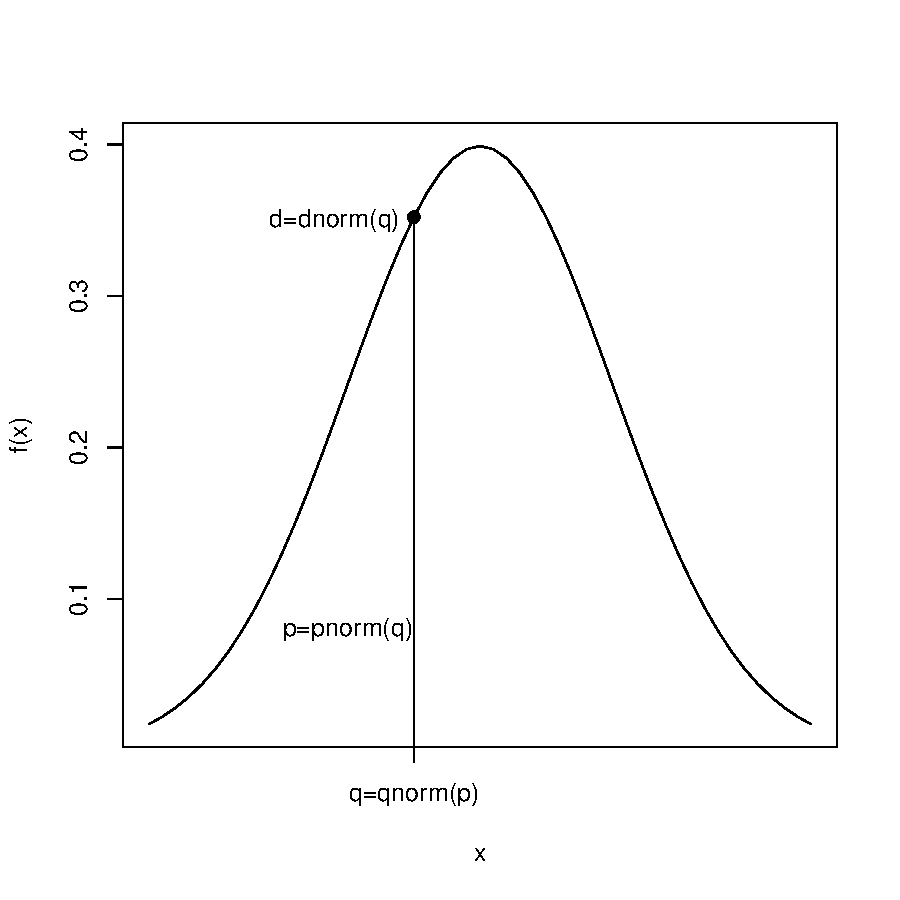
\includegraphics[width=3in, height=3in]{rslides-normal.pdf}
\end{figure}
\end{frame}

\begin{frame}[fragile]
\frametitle{final exercises}
Write up the following exercises into a \LaTeX\hspace{1pt} document.  Put any code you use into a {\tt verbatim} environment in the document.  All figures and tables should have captions and you should include a very short (1-2 sentence) writeup for everything you report describing what you did.
\bigskip
\begin{enumerate}
\item Load the {\tt PErisk} dataset from the {\tt Zelig} package.
\item Which country does the 35th observation belongs to?  Use code to identify the country.
\item Create a new dataset that omits Kenya from the dataset.
\item Using the new dataset, now extract the {\tt barb2} and {\tt gdpw2} variables.  Find the mean, median, standard deviation, and correlation of these two variables.  Present the results in a nicely formatted table in \LaTeX.
\end{enumerate}
\end{frame}

\begin{frame}[fragile]
\begin{enumerate}
\item[5.] Now let $\mathbf{X}$ be a matrix with two columns: the first column is a column of 1s and the second column is the {\tt gdpw2} variable.  Let $\mathbf{y}$ be the {\tt barb2} variable.  Create $\mathbf{X}$ and $\mathbf{y}$ and find $\bm{\hat{\beta}}$, where
\begin{eqnarray*}
 \bm{\hat{\beta}} = (\mathbf{X}^T\mathbf{X})^{-1} \mathbf{X}^T\mathbf{y}
\end{eqnarray*}
Type out this equation in \LaTeX\hspace{1pt} and also report the values in $\bm{\hat{\beta}}$.  $\bm{\hat{\beta}}$ should be a vector of length 2.  
\item[6.] Create two plots.  In the first plot, include the density of the {\tt gdpw2} and {\tt barb2} variables.  You should have two curves.  Differentiate the curves by color and/or type.  In the second plot, do a scatterplot with {\tt gdpw2} on the x-axis and {\tt barb2} on the y-axis.  Add a line that has an intercept at the first value of $\bm{\hat{\beta}}$ and a slope of the second value of $\bm{\hat{\beta}}$.  Include an informative legend for both plots.  Put these two plots side-by-side and include them as an image in your document.
\end{enumerate}
\end{frame}

\begin{frame}
\begin{itemize}
\item[7.] Write a function that takes in any $n \times k$ matrix for $\mathbf{X}$ and any $n \times 1$ vector for $\mathbf{y}$ and calculates $\bm{\hat{\beta}}$.
\item[8.] Do the following 1000 times with a for loop: Take a sample of 61 observations from the dataset with replacement.  For each sample, calculate $\bm{\hat{\beta}}$, where $\mathbf{X}$ and $\mathbf{y}$ are defined the same as in question 5.  Store your results in a $1000 \times 2$ matrix.
\item[9.]  Using the apply function, find and report the mean, standard deviation, and 2.5\% and 97.5\% quantiles for the two columns in your matrix.
\item[10.] For each column, draw 1000 draws from the normal distribution with the means and standard deviations from question 9.  That is, you should draw 1000 draws twice, once with the mean and sd from the first column and once with the mean and sd from the second column.  For each vector of 1000 draws, plot the density of the draws and include a vertical line for the mean of the draws.  You should be doing this twice, once for each set of the 1000 draws.  Include the two plots in your document.
\end{itemize}
\end{frame}

\begin{frame}[fragile]
\begin{enumerate}
\red
\footnotesize
\item
\begin{Schunk}
\begin{Sinput}
> library(Zelig)
> data(PErisk)
\end{Sinput}
\end{Schunk}
\item
\begin{Schunk}
\begin{Sinput}
> PErisk$country[35]
\end{Sinput}
\begin{Soutput}
[1] Malaysia
62 Levels: Argentina Australia Austria Bangladesh Belgium ... Zimbabwe
\end{Soutput}
\end{Schunk}
\item
\begin{Schunk}
\begin{Sinput}
> new.data <- PErisk[PErisk$country != "Kenya", ]
\end{Sinput}
\end{Schunk}
\item
\begin{Schunk}
\begin{Sinput}
> variables <- cbind(new.data$barb2, new.data$gdpw2)
> colMeans(variables)
\end{Sinput}
\begin{Soutput}
[1] -2.935360  9.065189
\end{Soutput}
\begin{Sinput}
> apply(variables, MARGIN = 2, FUN = sd)
\end{Sinput}
\begin{Soutput}
[1] 2.7285678 0.9606462
\end{Soutput}
\begin{Sinput}
> cor(new.data$barb2, new.data$gdpw2)
\end{Sinput}
\begin{Soutput}
[1] -0.5456426
\end{Soutput}
\end{Schunk}
\end{enumerate}
\end{frame}

\begin{frame}[fragile]
\begin{enumerate}
\red
\footnotesize
\item[5.]
\begin{Schunk}
\begin{Sinput}
> X <- cbind(1, new.data$gdpw2)
> y <- new.data$barb2
> beta.hat <- solve(t(X) %*% X) %*% t(X) %*% y
> beta.hat
\end{Sinput}
\begin{Soutput}
          [,1]
[1,] 11.113997
[2,] -1.549814
\end{Soutput}
\end{Schunk}
 
\item[6.]
\begin{Schunk}
\begin{Sinput}
> par(mfrow = c(1, 2))
> plot(density(new.data$gdpw2), xlab = "", ylab = "Density", 
+     main = "", xlim = c(-20, 20))
> lines(density(new.data$barb2), col = 2, lty = 2)
> legend(x = "topleft", legend = c("GDP", "Black Market Premium"), 
+     col = c(1, 2), lty = 1:2, cex = 0.5)
> plot(x = new.data$gdpw2, y = new.data$barb2, main = "", 
+     xlab = "GDP", ylab = "Black Market Premium")
> abline(a = beta.hat[1], b = beta.hat[2], col = 2)
> legend(x = "topright", legend = "Best Fit Line", col = 2, 
+     lty = 1, cex = 0.5)
\end{Sinput}
\end{Schunk}
\end{enumerate}
\end{frame}

\begin{frame}
 
\begin{center}
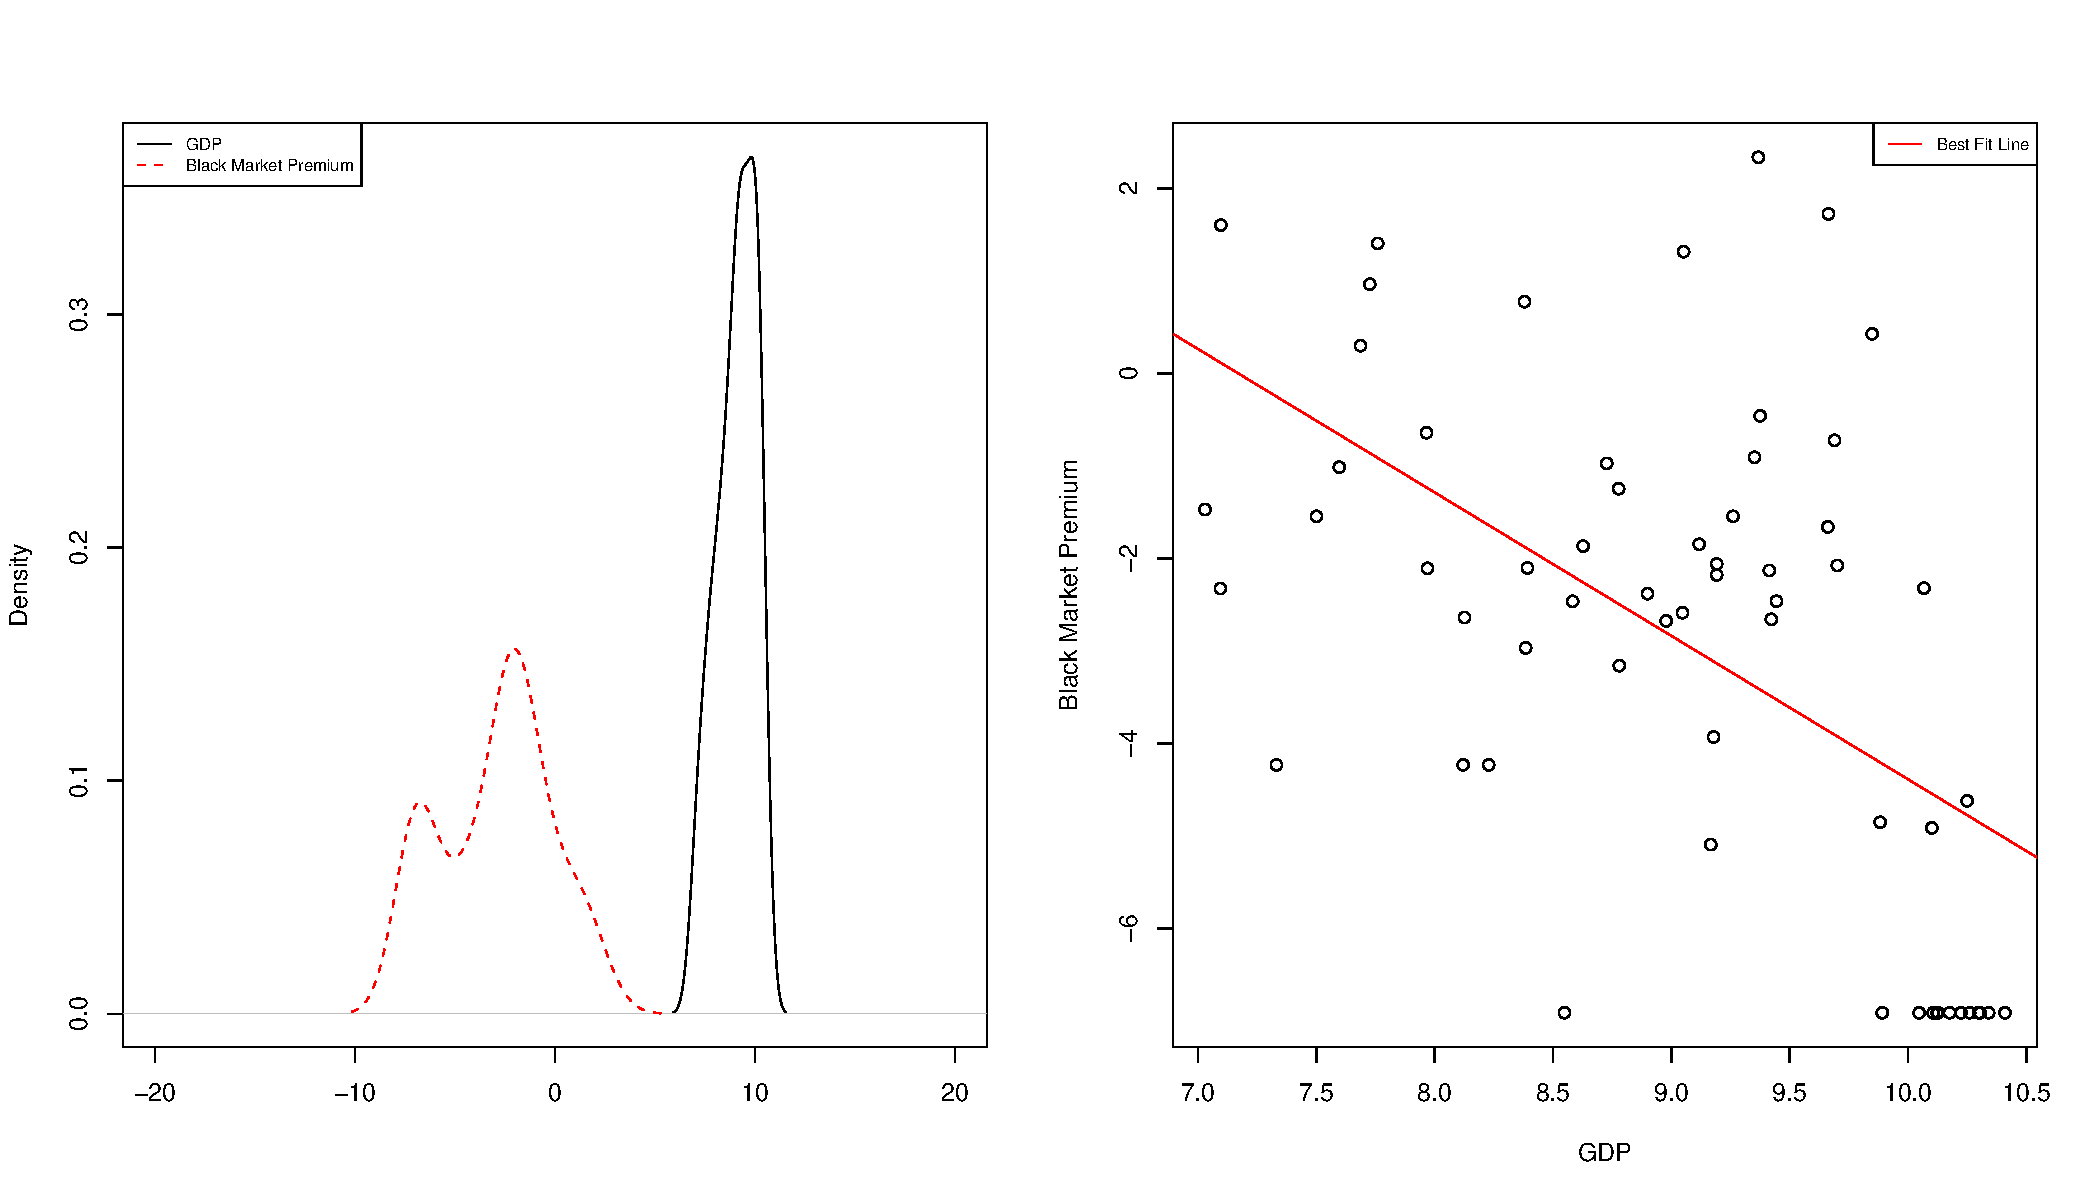
\includegraphics{rslides-plot6}
\end{center}
\end{frame}

\begin{frame}[fragile]
\begin{enumerate}
\red
\footnotesize
\item[7.]
\begin{Schunk}
\begin{Sinput}
> beta.func <- function(X, y) {
+     beta.hat <- solve(t(X) %*% X) %*% t(X) %*% y
+     return(beta.hat)
+ }
\end{Sinput}
\end{Schunk}
\item[8.]
\begin{Schunk}
\begin{Sinput}
> results <- matrix(NA, nrow=1000, ncol=2)
> for(i in 1:1000){
+   row.numbers <- sample(1:nrow(new.data), size=61, replace=T)
+   samp.data <- new.data[row.numbers,]  ## sample the data
+   X <- cbind(1, samp.data$gdpw2)
+   y <- samp.data$barb2
+   results[i,] <- beta.func(X=X, y=y)
+ }
\end{Sinput}
\end{Schunk}
\end{enumerate}
\end{frame}

\begin{frame}[fragile]
\begin{enumerate}
\red
\footnotesize
\item[9.]
\begin{Schunk}
\begin{Sinput}
> means <- apply(results, MARGIN = 2, FUN = mean)
> means
\end{Sinput}
\begin{Soutput}
[1] 11.157317 -1.552811
\end{Soutput}
\begin{Sinput}
> sds <- apply(results, MARGIN = 2, FUN = sd)
> sds
\end{Sinput}
\begin{Soutput}
[1] 2.6331276 0.2935984
\end{Soutput}
\begin{Sinput}
> quants <- apply(results, MARGIN = 2, FUN = quantile, probs = c(0.025, 
+     0.975))
> quants
\end{Sinput}
\begin{Soutput}
           [,1]       [,2]
2.5%   5.911529 -2.0948121
97.5% 16.090756 -0.9442727
\end{Soutput}
\end{Schunk}
\end{enumerate}
\end{frame}

\begin{frame}[fragile]
\begin{enumerate}
\red
\footnotesize
\item [10.]
\begin{center}
 
\begin{Schunk}
\begin{Sinput}
> first.draws <- rnorm(1000, mean = means[1], sd = sds[1])
> second.draws <- rnorm(1000, mean = means[2], sd = sds[2])
> par(mfrow = c(1, 2))
> plot(density(first.draws), xlab = expression(beta[1]), main = "")
> abline(v = mean(first.draws), col = 2)
> plot(density(second.draws), xlab = expression(beta[2]), 
+     main = "")
> abline(v = mean(second.draws), col = 2)
\end{Sinput}
\end{Schunk}
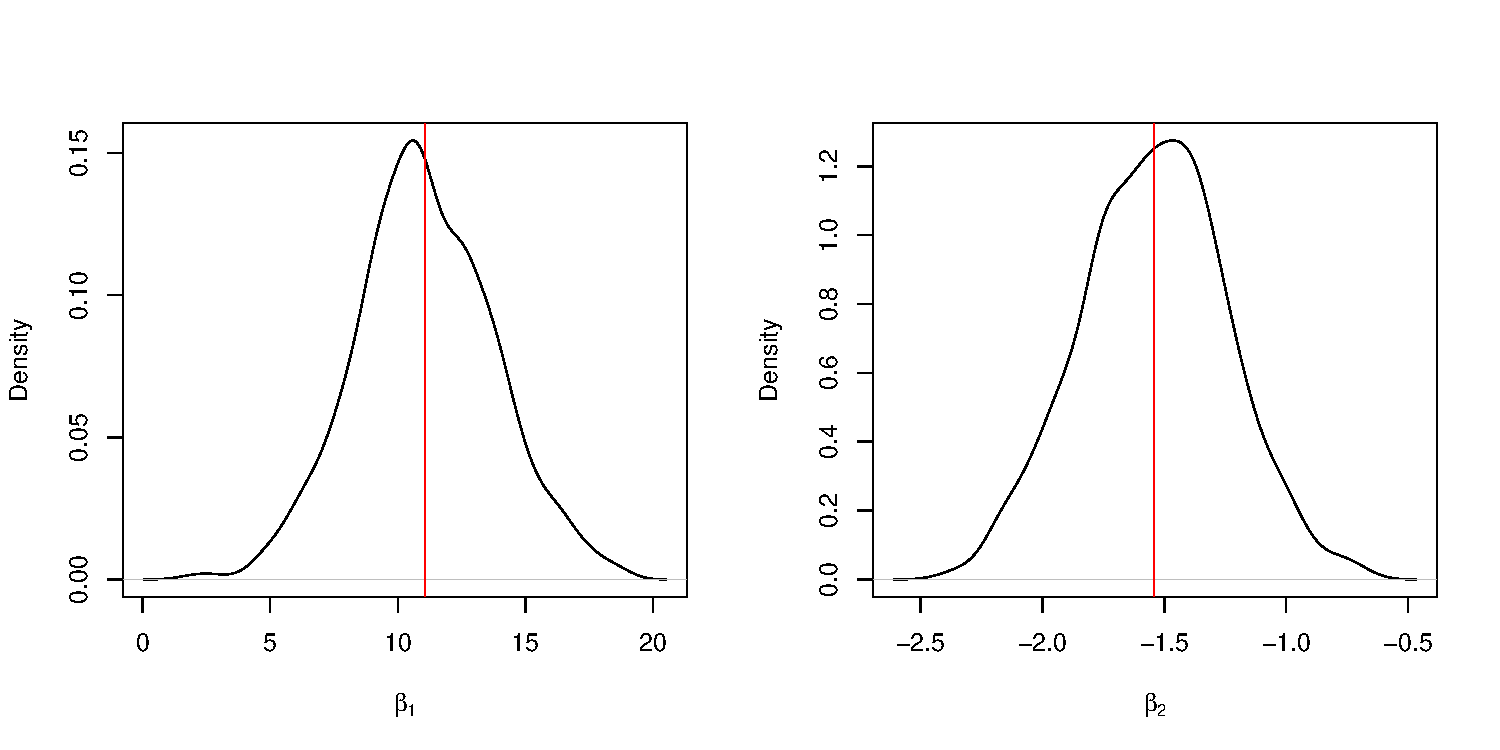
\includegraphics{rslides-plot7}
\end{center}
\end{enumerate}
\end{frame}
\end{document}



